\chapter{Higher Dimensional Eigenvalues}

In this chapter we verify the correctness and examine the performance of the Rayleigh quotient fixed point methods for higher-dimensional problems. We consider realistic two- and three-dimensional problems involving fuel rods and fuel assemblies. For higher dimensions, the phase space of the neutron transport equation is a function of two $(x, y)$ or three $(x, y, z)$ spatial variables and two $(\mu, \eta)$ or three $(\mu, \eta, \xi)$ angular variables defined as the $x$-, $y$-, and $z$-direction cosines. For higher-dimensional Cartesian geometry, the two-dimensional and three-dimensional alpha-eigenvalue neutron transport equations are given by Eq.~\ref{eq:2DAlpha} and Eq.~\ref{eq:3DAlpha}, respectively:

\begin{multline}
\bigg [ \mu \frac{\partial}{\partial x} + \eta \frac{\partial}{\partial y} + \frac{\alpha}{v(E)} + \sigma(x,y,E) \bigg ] \psi(x,y,\mu,\eta,E) \\ = \frac{\chi(E)}{2} \int_{0}^{\infty} \diff E' \nu(E') \sigma_{f}(x,y,E') \int_{-1}^{1} \diff \mu' \int_{-1}^{1} \diff \eta' \psi(x,y, \mu',\eta', E) \\ + \frac{1}{2\pi} \int_{0}^{\infty} \diff E' \sigma_{s}(x, y, E' \rightarrow E) \int_{-1}^{1} \diff \mu' \int_{-1}^{1} \diff \eta' \, \psi(x,y, \mu',\eta',E),
\label{eq:2DAlpha}
\end{multline}

\begin{multline}
\bigg [ \mu \frac{\partial}{\partial x} + \eta \frac{\partial}{\partial y} + \xi \frac{\partial}{\partial z} + \frac{\alpha}{v(E)} + \sigma(x,y,z,E) \bigg ] \psi(x,y,z,\mu,\eta,\xi, E) \\ = \frac{\chi(E)}{2} \int_{0}^{\infty} \diff E' \nu(E') \sigma_{f}(x,y,z,E') \int_{-1}^{1} \diff \mu' \int_{-1}^{1} \diff \eta' \int_{0}^{\pi} \diff \xi' \psi(x,y,z, \mu',\eta', \xi',E) \\ + \frac{1}{4\pi} \int_{0}^{\infty} \diff E' \sigma_{s}(x, y,z, E' \rightarrow E) \int_{-1}^{1} \diff \mu' \int_{-1}^{1} \diff \eta' \int_{0}^{\pi} \diff \xi' \, \psi(x,y,z, \mu',\eta',\xi',E),
\label{eq:3DAlpha}
\end{multline}

%Various homogeneous and heterogeneous slab geometry problems with vacuum boundary conditions were modeled in ARDRA. These slab media problems consist of multiplying and non-multiplying materials with thicknesses $\Delta$. Alpha- and $k$-effective eigenvalues were calculated and the number of transport sweeps compared to various methods such as the critical search method and the power method. To verify the correctness of the Rayleigh quotient fixed point method (RQFP), the method was compared to various methods such as Green's Function Method (GFM) and Direct Evaluation (DE) and compared to other discrete ordinate neutron transport codes such as PARTISN/DANT.

\section{Cylinder Benchmark Problems}

\begin{figure}[!htbp]
	\centering
	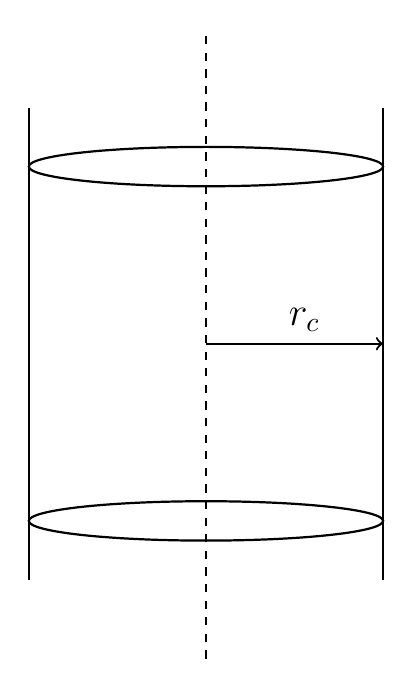
\begin{tikzpicture}[text centered]
    \begin{scope}[thick,font=\Large]

    \draw [-] (-2.25,-3) -- (-2.25,3) {};
%    \draw [-] (2.5,-3) -- (0.5,3) {};
    
    \draw [dashed] (0.0,-4) -- (0,4) {};
    \draw (2.25,-3.) -- (2.25,3) {};
    
    \draw [->] (0,0) -- (2.25,0) node [align=center] at (1.25,0.3) {$r_{c}$};
    
    \draw (0,2.25) ellipse (2.25 and 0.25);
    \draw (0,-2.25) ellipse (2.25 and 0.25);

    \end{scope}
\end{tikzpicture}
	\caption{Critical Radius of Infinite Cylinder}
	\label{fig:CylCritRadius}
\end{figure}

\begin{table}[!htbp]
	\caption{One-Group Cross Sections for Infinite Cylinder Critical Problems (cm$^{-1}$) \cite{sood2003analytical}}
	\label{table:SoodCyl}
	\centering\ra{1.3}
    \begin{tabular}{*6c}
        \toprule
	Cross Section Set & $\sigma$ & $\nu \sigma_{f}$ & $\sigma_{s0}$ & $\sigma_{s1}$ & $v$ [cm/s] \\ 
        \midrule
	PUb & 0.32640 & 0.231744 & 0.225216 & 0.0 & 1 \\
	U-235a & 0.32640 & 0.176256 & 0.248064 & 0.0 & 1 \\
	U-D$_{2}$O & 0.54628 & 0.0928676 & 0.464338 & 0.0 & 1 \\
	U-235a Anisotropic & 0.32640 & 1.76256 & 0.248064 & 0.04432 & 1 \\
	U-235b Anisotropic & 0.32640 & 1.76256 & 0.248064 & 0.212160 & 1 \\
        \bottomrule
    \end{tabular}
\end{table}

\begin{table}[!htbp]
	\caption{Calculated Eigenvalues and Transport Sweep Comparisons for Critical Infinite Cylinder Problems in \cite{sood2003analytical}}
	\label{table:SoodCyl}
	\begin{subtable}[h]{1.0\textwidth}
	\centering\ra{1.3}
	\begin{tabular}{@{}ccccc@{}}\toprule
	& & & \multicolumn{2}{c}{Transport Sweeps} \\
	\cmidrule{4-5} Cross Section Set & r$_{c}$ [cm] & Calculated $\alpha$ [s$^{-1}$] & RQFP & Critical Search\\
	\midrule
	PUb & 4.279960 & $3.783833 \times 10^{-4}$ & 38 & 461 \\
	U-235a & 5.284935 & $ 1.973082 \times 10^{-4}$ & 45 & 455 \\
	U-D$_{2}$O & 16.554249 & $ -1.007328 \times 10^{-4}$ &  319 & * \\
	U-235a Anisotropic & 5.514296811 & $ 6.549139 \times 10^{-3}$ & 47 & 99260 \\
	U-235b Anisotropic (Check this) & 6.940205668 & $ 6.549139 \times 10^{-3}$ & 47 & 99260 \\ 
	\bottomrule
	\multicolumn{5}{l}{*Did Not Converge} \\
	\end{tabular}
	\caption{Alpha-Eigenvalue: Comparison of RQFP and Critical Search Transport Sweeps}
	\label{table:SoodCylAlpha}
	\end{subtable}%
	\vspace{0.25cm}
	\begin{subtable}[h]{1.0\textwidth}
	\centering\ra{1.3}
	\begin{tabular}{@{}ccccc@{}}\toprule
	& & \multicolumn{2}{c}{Transport Sweeps} \\
	\cmidrule{4-5} Cross Section Set & r$_{c}$ [cm] & Reference $k_{\text{eff}}$ & RQFP & Power Method \\
	\midrule
	PUb & 4.279960 & 1.001419 & 43 & 40 \\
	U-235a & 5.284935 & 1.000989 & 49 & 42 \\
	U-D$_{2}$O & 16.554249 & 0.998935 & 320 & 121 \\
	U-235a Anisotropic & 5.514296811 & 1.034070 & 51 & 43 \\
	U-235b Anisotropic (Check this) & 6.940205668 &  &  & \\
	\bottomrule
	\multicolumn{5}{l}{$M = 500$, $L = 10$, Tolerance = $10^{-12}$} \\
	\end{tabular}
	\caption{$k$-Effective: Comparison of RQFP and Power Method Transport Sweeps}
	\label{table:SoodCylK}
	\end{subtable}
\end{table}

\section{Two- and Three-Dimensional Cartesian Benchmark Problems}

\begin{figure}
\begin{table}[H]
	\begin{subtable}[h]{1.0\textwidth}
    \centering
    \caption{UO$_{2}$ Fuel-Clad Cross Sections --  (cm$^{-1}$)}
    \resizebox{1.00\textwidth}{!}{
    \begin{tabular}{*8c}
        \toprule
	Energy Group $g$ & $\sigma_{g}$ & $\sigma_{g,tr}$ & $\sigma_{a,g}$ & $\sigma_{\gamma,g}$ & $\sigma_{f,g}$ & $\nu_{g}$ & $\chi_{g}$ \\ 
        \midrule
1 & 2.12450E-01 & 1.77949E-01 & 8.02480E-03 & 8.12740E-04 & 7.21206E-03 & 2.78145E+00 & 5.87910E-01 \\
2 & 3.55470E-01 & 3.29805E-01 & 3.71740E-03 & 2.89810E-03 & 8.19301E-04 & 2.47443E+00 & 4.11760E-01 \\
3 & 4.85540E-01 & 4.80388E-01 & 2.67690E-02 & 2.03158E-02 & 6.45320E-03 & 2.43383E+00 & 3.39060E-04 \\
4 & 5.59400E-01 & 5.54367E-01 & 9.62360E-02 & 7.76712E-02 & 1.85648E-02 & 2.43380E+00 & 1.17610E-07 \\
5 & 3.18030E-01 & 3.11801E-01 & 3.00200E-02 & 1.22116E-02 & 1.78084E-02 & 2.43380E+00 & 0.00000E+00 \\
6 & 4.01460E-01 & 3.95168E-01 & 1.11260E-01 & 2.82252E-02 & 8.30348E-02 & 2.43380E+00 & 0.00000E+00 \\
7 & 5.70610E-01 & 5.64406E-01 & 2.82780E-01 & 6.67760E-02 & 2.16004E-01 & 2.43380E+00 & 0.00000E+00 \\
        \bottomrule
        & & & & & & & 
    \end{tabular}}
 \end{subtable} %
%\end{table}
\begin{subtable}[h]{1.0\textwidth}
%\begin{table}[H]
    \centering
    \caption{UO$_{2}$ Fuel-Clad Scattering Block (cm$^{-1}$)}
    \resizebox{1.00\textwidth}{!}{
    \begin{tabular}{*8c}
        \toprule
	$g'$, $g$ & 1 & 2 & 3 & 4 & 5 & 6 & 7 \\
        \midrule
1 & 1.27537E-01 & 4.23780E-02 & 9.43740E-06 & 5.51630E-09 & 0.00000E+00 & 0.00000E+00 & 0.00000E+00 \\
2 & 0.00000E+00 & 3.24456E-01 & 1.63140E-03 & 3.14270E-09 & 0.00000E+00 & 0.00000E+00 & 0.00000E+00 \\
3 & 0.00000E+00 & 0.00000E+00 & 4.50940E-01 & 2.67920E-03 & 0.00000E+00 & 0.00000E+00 & 0.00000E+00 \\
4 & 0.00000E+00 & 0.00000E+00 & 0.00000E+00 & 4.52565E-01 & 5.56640E-03 & 0.00000E+00 & 0.00000E+00 \\
5 & 0.00000E+00 & 0.00000E+00 & 0.00000E+00 & 1.25250E-04 & 2.71401E-01 & 1.02550E-02 & 1.00210E-08 \\
6 & 0.00000E+00 & 0.00000E+00 & 0.00000E+00 & 0.00000E+00 & 1.29680E-03 & 2.65802E-01 & 1.68090E-02 \\
7 & 0.00000E+00 & 0.00000E+00 & 0.00000E+00 & 0.00000E+00 & 0.00000E+00 & 8.54580E-03 & 2.73080E-01 \\
        \bottomrule
        & & & & & & & 
    \end{tabular}}
  \end{subtable}
    \caption{C5G7MOX Cross Sections - UO$_{2}$ Fuel-Clad}
\end{table}
\end{figure}
\begin{figure}
\begin{table}[H]
  \begin{subtable}[h]{1.0\textwidth}
%\begin{table}[H]
    \centering
    \caption{4.3\% MOX Fuel -- Clad Cross Sections (cm$^{-1}$)}
    \resizebox{1.00\textwidth}{!}{
    \begin{tabular}{*8c}
        \toprule
	Energy Group $g$ & $\sigma_{g}$ & $\sigma_{g,tr}$ & $\sigma_{a,g}$ & $\sigma_{\gamma,g}$ & $\sigma_{f,g}$ & $\nu_{g}$ & $\chi_{g}$ \\ 
        \midrule
1 & 2.11920E-01	 &	1.78731E-01 &	8.43390E-03 &	8.06860E-04 &	7.62704E-03 &	2.85209E+00 &	5.87910E-01 \\
2 & 3.55810E-01	 &	3.30849E-01 &	3.75770E-03 &	2.88080E-03 &	8.76898E-04 &	2.89099E+00 &	4.11760E-01 \\
3 & 4.88900E-01	 &	4.83772E-01 &	2.79700E-02 &	2.22717E-02 &	5.69835E-03 &	2.85486E+00 &	3.39060E-04 \\
4 & 5.71940E-01	 &	5.66922E-01 &	1.04210E-01 &	8.13228E-02 &	2.28872E-02 &	2.86073E+00 &	1.17610E-07 \\
5 & 4.32390E-01	 &	4.26227E-01 &	1.39940E-01 &	1.29177E-01 &	1.07635E-02 &	2.85447E+00 &	0.00000E+00 \\
6 & 6.84950E-01	 &	6.78997E-01 &	4.09180E-01 &	1.76423E-01 &	2.32757E-01 &	2.86415E+00 &	0.00000E+00 \\
7 & 6.88910E-01	 &	6.82852E-01 &	4.09350E-01 &	1.60382E-01 &	2.48968E-01 &	2.86780E+00 &	0.00000E+00 \\
        \bottomrule
        & & & & & & & 
    \end{tabular}}
  \end{subtable}
  \begin{subtable}[h]{1.0\textwidth}
%\begin{table}[H]
    \centering
    \caption{4.3\% MOX Fuel Scattering Block (cm$^{-1}$)}
    \resizebox{1.00\textwidth}{!}{
    \begin{tabular}{*8c}
        \toprule
	$g'$, $g$ & 1 & 2 & 3 & 4 & 5 & 6 & 7 \\
        \midrule
1 & 1.28876E-01	 &	4.14130E-02 &	8.22900E-06 &	5.04050E-09 &	0.00000E+00 &	0.00000E+00 &	0.00000E+00 \\
2 & 0.00000E+00	 &	3.25452E-01 &	1.63950E-03 &	1.59820E-09 &	0.00000E+00 &	0.00000E+00 &	0.00000E+00 \\
3 & 0.00000E+00	 &	0.00000E+00 &	4.53188E-01 &	2.61420E-03 &	0.00000E+00 &	0.00000E+00 &	0.00000E+00 \\
4 & 0.00000E+00	 &	0.00000E+00 &	0.00000E+00 &	4.57173E-01 &	5.53940E-03 &	0.00000E+00 &	0.00000E+00 \\
5 & 0.00000E+00	 &	0.00000E+00 &	0.00000E+00 &	1.60460E-04 &	2.76814E-01 &	9.31270E-03 &	9.16560E-09 \\
6 & 0.00000E+00	 &	0.00000E+00 &	0.00000E+00 &	0.00000E+00 &	2.00510E-03 &	2.52962E-01 &	1.48500E-02 \\
7 & 0.00000E+00	 &	0.00000E+00 &	0.00000E+00 &	0.00000E+00 &	0.00000E+00 &	8.49480E-03 &	2.65007E-01 \\
        \bottomrule
        & & & & & & & 
    \end{tabular}}
  \end{subtable}
    \caption{C5G7MOX Cross Sections - 4.3\% MOX Fuel}
\end{table}
\end{figure}

\begin{figure}
\begin{table}[H]
    \begin{subtable}[h]{1.0\textwidth}
%\begin{table}[H]
    \centering
    \caption{7.0\% MOX Fuel -- Clad Cross Sections (cm$^{-1}$)}
    \resizebox{1.00\textwidth}{!}{
    \begin{tabular}{*8c}
        \toprule
	Energy Group $g$ & $\sigma_{g}$ & $\sigma_{g,tr}$ & $\sigma_{a,g}$ & $\sigma_{\gamma,g}$ & $\sigma_{f,g}$ & $\nu_{g}$ & $\chi_{g}$ \\ 
        \midrule
1 &	2.14540E-01	 &	1.81323E-01 &	9.06570E-03 &	8.11240E-04 &	8.25446E-03 &	2.88498E+00 &	5.87910E-01 \\
2 &	3.59350E-01	 &	3.34368E-01 &	4.29670E-03 &	2.97105E-03 &	1.32565E-03 &	2.91079E+00 &	4.11760E-01 \\
3 &	4.98910E-01	 &	4.93785E-01 &	3.28810E-02 &	2.44594E-02 &	8.42156E-03 &	2.86574E+00 &	3.39060E-04 \\
4 &	5.96220E-01	 &	5.91216E-01 &	1.22030E-01 &	8.91570E-02 &	3.28730E-02 &	2.87063E+00 &	1.17610E-07 \\
5 &	4.80350E-01	 &	4.74198E-01 &	1.82980E-01 &	1.67016E-01 &	1.59636E-02 &	2.86714E+00 &	0.00000E+00 \\
6 &	8.39360E-01	 &	8.33601E-01 &	5.68460E-01 &	2.44666E-01 &	3.23794E-01 &	2.86658E+00 &	0.00000E+00 \\
7 &	8.59480E-01	 &	8.53603E-01 &	5.85210E-01 &	2.22407E-01 &	3.62803E-01 &	2.87539E+00 &	0.00000E+00 \\
        \bottomrule
        & & & & & & & 
    \end{tabular}}
  \end{subtable}
  \begin{subtable}[h]{1.0\textwidth}
%\begin{table}[H]
    \centering
    \caption{7.0\% MOX Fuel Scattering Block (cm$^{-1}$)}
    \resizebox{1.00\textwidth}{!}{
    \begin{tabular}{*8c}
        \toprule
	$g'$, $g$ & 1 & 2 & 3 & 4 & 5 & 6 & 7 \\
        \midrule
1 &	1.30457E-01	 &	4.17920E-02 &	8.51050E-06 &	5.13290E-09 &	0.00000E+00 &	0.00000E+00 &	0.00000E+00 \\
2 &	0.00000E+00	 &	3.28428E-01 &	1.64360E-03 &	2.20170E-09 &	0.00000E+00 &	0.00000E+00 &	0.00000E+00 \\
3 &	0.00000E+00	 &	0.00000E+00 &	4.58371E-01 &	2.53310E-03 &	0.00000E+00 &	0.00000E+00 &	0.00000E+00 \\
4 &	0.00000E+00	 &	0.00000E+00 &	0.00000E+00 &	4.63709E-01 &	5.47660E-03 &	0.00000E+00 &	0.00000E+00 \\
5 &	0.00000E+00	 &	0.00000E+00 &	0.00000E+00 &	1.76190E-04 &	2.82313E-01 &	8.72890E-03 &	9.00160E-09 \\
6 &	0.00000E+00	 &	0.00000E+00 &	0.00000E+00 &	0.00000E+00 &	2.27600E-03 &	2.49751E-01 &	1.31140E-02 \\
7 &	0.00000E+00	 &	0.00000E+00 &	0.00000E+00 &	0.00000E+00 &	0.00000E+00 &	8.86450E-03 &	2.59529E-01 \\
        \bottomrule
        & & & & & & & 
    \end{tabular}}
  \end{subtable}
  \caption{C5G7MOX Cross Sections - 7.0\% MOX Fuel}
\end{table}
\end{figure}

\begin{figure}
\begin{table}[H]
    \begin{subtable}[h]{1.0\textwidth}
%\begin{table}[H]
    \centering
    \caption{8.7\% MOX Fuel -- Clad Cross Sections (cm$^{-1}$)}
    \resizebox{1.00\textwidth}{!}{
    \begin{tabular}{*8c}
        \toprule
	Energy Group $g$ & $\sigma_{g}$ & $\sigma_{g,tr}$ & $\sigma_{a,g}$ & $\sigma_{\gamma,g}$ & $\sigma_{f,g}$ & $\nu_{g}$ & $\chi_{g}$ \\ 
        \midrule
1 &	2.16280E-01	 &	1.83045E-01 &	9.48620E-03 &	8.14110E-04 &	8.67209E-03 &	2.90426E+00 &	5.87910E-01 \\
2 &	3.61700E-01	 &	3.36705E-01 &	4.65560E-03 &	3.03134E-03 &	1.62426E-03 &	2.91795E+00 &	4.11760E-01 \\
3 &	5.05630E-01	 &	5.00507E-01 &	3.62400E-02 &	2.59684E-02 &	1.02716E-02 &	2.86986E+00 &	3.39060E-04 \\
4 &	6.11170E-01	 &	6.06174E-01 &	1.32720E-01 &	9.36753E-02 &	3.90447E-02 &	2.87491E+00 &	1.17610E-07 \\
5 &	5.08900E-01	 &	5.02754E-01 &	2.08400E-01 &	1.89142E-01 &	1.92576E-02 &	2.87175E+00 &	0.00000E+00 \\
6 &	9.26670E-01	 &	9.21028E-01 &	6.58700E-01 &	2.83812E-01 &	3.74888E-01 &	2.86752E+00 &	0.00000E+00 \\
7 &	9.60990E-01	 &	9.55231E-01 &	6.90170E-01 &	2.59571E-01 &	4.30599E-01 &	2.87808E+00 &	0.00000E+00 \\
        \bottomrule
        & & & & & & & 
    \end{tabular}}
  \end{subtable}
  \begin{subtable}[h]{1.0\textwidth}
%\begin{table}[H]
    \centering
    \caption{8.7\% MOX Fuel Scattering Block (cm$^{-1}$)}
    \resizebox{1.00\textwidth}{!}{
    \begin{tabular}{*8c}
        \toprule
	$g'$, $g$ & 1 & 2 & 3 & 4 & 5 & 6 & 7 \\
        \midrule
1 &	1.31504E-01 &	4.20460E-02 &	8.69720E-06	& 5.19380E-09	& 0.00000E+00	& 0.00000E+00	& 0.00000E+00 \\
2 &	0.00000E+00 &	3.30403E-01 &	1.64630E-03	& 2.60060E-09	& 0.00000E+00	& 0.00000E+00	& 0.00000E+00 \\
3 &	0.00000E+00 &	0.00000E+00 &	4.61792E-01	& 2.47490E-03	& 0.00000E+00	& 0.00000E+00	& 0.00000E+00 \\
4 &	0.00000E+00 &	0.00000E+00 &	0.00000E+00	& 4.68021E-01	& 5.43300E-03	& 0.00000E+00	& 0.00000E+00 \\
5 &	0.00000E+00 &	0.00000E+00 &	0.00000E+00	& 1.85970E-04	& 2.85771E-01	& 8.39730E-03	& 8.92800E-09 \\
6 &	0.00000E+00 &	0.00000E+00 &	0.00000E+00	& 0.00000E+00	& 2.39160E-03	& 2.47614E-01	& 1.23220E-02 \\
7 &	0.00000E+00 &	0.00000E+00 &	0.00000E+00	& 0.00000E+00	& 0.00000E+00	& 8.96810E-03	& 2.56093E-01 \\
        \bottomrule
        & & & & & & & 
    \end{tabular}}
  \end{subtable}
  \caption{C5G7MOX Cross Sections - 8.7\% MOX Fuel}
\end{table}
\end{figure}

\begin{figure}
\begin{table}[H]
    \begin{subtable}[h]{1.0\textwidth}
%\begin{table}[H]
    \centering
    \caption{Fission Chamber -- Cross Sections (cm$^{-1}$)}
    \resizebox{1.00\textwidth}{!}{
    \begin{tabular}{*8c}
        \toprule
	Energy Group $g$ & $\sigma_{g}$ & $\sigma_{g,tr}$ & $\sigma_{a,g}$ & $\sigma_{\gamma,g}$ & $\sigma_{f,g}$ & $\nu_{g}$ & $\chi_{g}$ \\ 
        \midrule
1 &	1.90730E-01	&	1.26032E-01 &	5.11320E-04 &	5.11315E-04 &	4.79002E-09 &	2.76283E+00	& 5.87910E-01 \\
2 &	4.56520E-01	&	2.93160E-01 &	7.58130E-05 &	7.58072E-05 &	5.82564E-09 &	2.46239E+00	& 4.11760E-01 \\
3 &	6.40700E-01	&	2.84250E-01 &	3.16430E-04 &	3.15966E-04 &	4.63719E-07 &	2.43380E+00	& 3.39060E-04 \\
4 &	6.49840E-01	&	2.81020E-01 &	1.16750E-03 &	1.16226E-03 &	5.24406E-06 &	2.43380E+00	& 1.17610E-07 \\
5 &	6.70630E-01	&	3.34460E-01 &	3.39770E-03 &	3.39755E-03 &	1.45390E-07 &	2.43380E+00	& 0.00000E+00 \\
6 &	8.75060E-01	&	5.65640E-01 &	9.18860E-03 &	9.18789E-03 &	7.14972E-07 &	2.43380E+00	& 0.00000E+00 \\
7 &	1.43450E+00	&	1.17214E+00 &	2.32440E-02 &	2.32419E-02 &	2.08041E-06 &	2.43380E+00	& 0.00000E+00 \\
        \bottomrule
        & & & & & & & 
    \end{tabular}}
  \end{subtable}
  \begin{subtable}[h]{1.0\textwidth}
%\begin{table}[H]
    \centering
    \caption{Fission Chamber Scattering Block (cm$^{-1}$)}
    \resizebox{1.00\textwidth}{!}{
    \begin{tabular}{*8c}
        \toprule
	$g'$, $g$ & 1 & 2 & 3 & 4 & 5 & 6 & 7 \\
        \midrule
1 &	6.61659E-02 &	5.90700E-02 &	2.83340E-04 &	1.46220E-06 &	2.06420E-08 &	0.00000E+00 &	0.00000E+00 \\
2 &	0.00000E+00 &	2.40377E-01 &	5.24350E-02 &	2.49900E-04 &	1.92390E-05 &	2.98750E-06 &	4.21400E-07 \\
3 &	0.00000E+00 &	0.00000E+00 &	1.83425E-01 &	9.22880E-02 &	6.93650E-03 &	1.07900E-03 &	2.05430E-04 \\
4 &	0.00000E+00 &	0.00000E+00 &	0.00000E+00 &	7.90769E-02 &	1.69990E-01 &	2.58600E-02 &	4.92560E-03 \\
5 &	0.00000E+00 &	0.00000E+00 &	0.00000E+00 &	3.73400E-05 &	9.97570E-02 &	2.06790E-01 &	2.44780E-02 \\
6 &	0.00000E+00 &	0.00000E+00 &	0.00000E+00 &	0.00000E+00 &	9.17420E-04 &	3.16774E-01 &	2.38760E-01 \\
7 &	0.00000E+00 &	0.00000E+00 &	0.00000E+00 &	0.00000E+00 &	0.00000E+00 &	4.97930E-02 &	1.09910E+00 \\
        \bottomrule
        & & & & & & & 
    \end{tabular}}
  \end{subtable}
  \caption{C5G7MOX Cross Sections - Fission Chamber}
\end{table}
\end{figure}

\begin{figure}
\begin{table}[H]
    \begin{subtable}[h]{1.0\textwidth}
%\begin{table}[H]
    \centering
    \caption{Guide Tube Cross Sections (cm$^{-1}$)}
    \resizebox{1.00\textwidth}{!}{
    \begin{tabular}{*5c}
        \toprule
	Energy Group $g$ & $\sigma_{g}$ & $\sigma_{g,tr}$ & $\sigma_{a,g}$ & $\sigma_{\gamma,g}$ \\ 
        \midrule
1 &	1.90730E-01 &	1.26032E-01 &	5.11320E-04 &	5.11320E-04 \\
2 &	4.56520E-01 &	2.93160E-01 &	7.58010E-05 &	7.58010E-05 \\
3 &	6.40670E-01 &	2.84240E-01 &	3.15720E-04 &	3.15720E-04 \\
4 &	6.49670E-01 &	2.80960E-01 &	1.15820E-03 &	1.15820E-03 \\
5 &	6.70580E-01 &	3.34440E-01 &	3.39750E-03 &	3.39750E-03 \\
6 &	8.75050E-01 &	5.65640E-01 &	9.18780E-03 &	9.18780E-03 \\
7 &	1.43450E+00 &	1.17215E+00 &	2.32420E-02 &	2.32420E-02 \\
        \bottomrule
        & & & &
    \end{tabular}}
  \end{subtable}
  \begin{subtable}[h]{1.0\textwidth}
%\begin{table}[H]
    \centering
    \caption{Guide Tube Scattering Block (cm$^{-1}$)}
    \resizebox{1.00\textwidth}{!}{
    \begin{tabular}{*8c}
        \toprule
	$g'$, $g$ & 1 & 2 & 3 & 4 & 5 & 6 & 7 \\
        \midrule
1	& 6.61659E-02 &	5.90700E-02 &	2.83340E-04 &	1.46220E-06 &	2.06420E-08 &	0.00000E+00 &	0.00000E+00 \\
2	& 0.00000E+00 &	2.40377E-01 &	5.24350E-02 &	2.49900E-04 &	1.92390E-05 &	2.98750E-06 &	4.21400E-07 \\
3	& 0.00000E+00 &	0.00000E+00 &	1.83297E-01 &	9.23970E-02 &	6.94460E-03 &	1.08030E-03 &	2.05670E-04 \\
4	& 0.00000E+00 &	0.00000E+00 &	0.00000E+00 &	7.88511E-02 &	1.70140E-01 &	2.58810E-02 &	4.92970E-03 \\
5	& 0.00000E+00 &	0.00000E+00 &	0.00000E+00 &	3.73330E-05 &	9.97372E-02 &	2.06790E-01 &	2.44780E-02 \\
6	& 0.00000E+00 &	0.00000E+00 &	0.00000E+00 &	0.00000E+00 &	9.17260E-04 &	3.16765E-01 &	2.38770E-01 \\
7	& 0.00000E+00 &	0.00000E+00 &	0.00000E+00 &	0.00000E+00 &	0.00000E+00 &	4.97920E-02 &	1.09912E+00 \\
        \bottomrule
        & & & & & & & 
    \end{tabular}}
  \end{subtable}
  \caption{C5G7MOX Cross Sections - Guide Tube}
\end{table}
\end{figure}

\begin{figure}
\begin{table}[H]
    \begin{subtable}[h]{1.0\textwidth}
%\begin{table}[H]
    \centering
    \caption{Moderator Cross Sections (cm$^{-1}$)}
    \resizebox{1.00\textwidth}{!}{
    \begin{tabular}{*5c}
        \toprule
	Energy Group $g$ & $\sigma_{g}$ & $\sigma_{g,tr}$ & $\sigma_{a,g}$ & $\sigma_{\gamma,g}$ \\ 
        \midrule
1 &	2.30070E-01  &	1.59206E-01  &	6.01050E-04  &	6.01050E-04 \\
2 &	7.76460E-01  &	4.12970E-01  &	1.57930E-05  &	1.57930E-05 \\
3 &	1.48420E+00  &	5.90310E-01  &	3.37160E-04  &	3.37160E-04 \\
4 &	1.50520E+00  &	5.84350E-01  &	1.94060E-03  &	1.94060E-03 \\
5 &	1.55920E+00  &	7.18000E-01  &	5.74160E-03  &	5.74160E-03 \\
6 &	2.02540E+00  &	1.25445E+00  &	1.50010E-02  &	1.50010E-02 \\
7 &	3.30570E+00  &	2.65038E+00  &	3.72390E-02  &	3.72390E-02 \\
        \bottomrule
        & & & &
    \end{tabular}}
  \end{subtable}
  \begin{subtable}[h]{1.0\textwidth}
%\begin{table}[H]
    \centering
    \caption{Moderator Scattering Block (cm$^{-1}$)}
    \resizebox{1.00\textwidth}{!}{
    \begin{tabular}{*8c}
        \toprule
	$g'$, $g$ & 1 & 2 & 3 & 4 & 5 & 6 & 7 \\
        \midrule
1 &	4.44777E-02  &	1.13400E-01  &	7.23470E-04  &	3.74990E-06  &	5.31840E-08  &	0.00000E+00  &	0.00000E+00 \\
2 &	0.00000E+00  &	2.82334E-01  &	1.29940E-01  &	6.23400E-04  &	4.80020E-05  &	7.44860E-06  &	1.04550E-06 \\
3 &	0.00000E+00  &	0.00000E+00  &	3.45256E-01  &	2.24570E-01  &	1.69990E-02  &	2.64430E-03  &	5.03440E-04 \\
4 &	0.00000E+00  &	0.00000E+00  &	0.00000E+00  &	9.10284E-02  &	4.15510E-01  &	6.37320E-02  &	1.21390E-02 \\
5 &	0.00000E+00  &	0.00000E+00  &	0.00000E+00  &	7.14370E-05  &	1.39138E-01  &	5.11820E-01  &	6.12290E-02 \\
6 &	0.00000E+00  &	0.00000E+00  &	0.00000E+00  &	0.00000E+00  &	2.21570E-03  &	6.99913E-01  &	5.37320E-01 \\
7 &	0.00000E+00  &	0.00000E+00  &	0.00000E+00  &	0.00000E+00  &	0.00000E+00  &	1.32440E-01  &	2.48070E+00 \\
        \bottomrule
        & & & & & & & 
    \end{tabular}}
  \end{subtable}
  \caption{C5G7MOX Cross Sections - Moderator}
\end{table}
\end{figure}

\section{Conclusion}